%% Dokumentenvorspann f�r Aufgabenblatt Friesen Freitage
%%
%% (c) 2008 Carsten Lynker
%%
%% Abgeleitet aus einer fr�heren Klassenarbeitsvorlage
%%
%% Die einzelnen Aufgaben sind mit \aufgabe einzuleiten, die
%% Aufz�hlungsumgebung enumerate hat die in Klassenarbeiten
%% �bliche Form a) ... b) ...
%%

\documentclass[11pt,parskip=half,a4paper]{scrartcl}
%\usepackage{ngerman}
\usepackage[latin9]{inputenc}
\usepackage[T1]{fontenc}
\usepackage{multicol}
\usepackage{graphicx}
\usepackage{pslatex}
\usepackage{helvet}
\usepackage{listings}
\lstset{numbers=left, numberstyle=\tiny, numbersep=4pt, breaklines=true, frame=single, showstringspaces=false, basicstyle=\scriptsize}
% -*- latex -*-
% Definition of the Lua language for the listings package
% Time-stamp: <2008-11-30 15:27:16 rsmith>
% Written by Roland Smith <rsmith@xs4all.nl> and hereby placed in the public
% domain. 

\lstdefinelanguage{lua}
  {morekeywords={and,break,do,else,elseif,end,false,for,function,if,in,local,
     nil,not,or,repeat,return,then,true,until,while},
   morekeywords={[2]arg,assert,collectgarbage,dofile,error,_G,getfenv,
     getmetatable,ipairs,load,loadfile,loadstring,next,pairs,pcall,print,
     rawequal,rawget,rawset,select,setfenv,setmetatable,tonumber,tostring,
     type,unpack,_VERSION,xpcall},
   morekeywords={[2]coroutine.create,coroutine.resume,coroutine.running,
     coroutine.status,coroutine.wrap,coroutine.yield},
   morekeywords={[2]module,require,package.cpath,package.load,package.loaded,
     package.loaders,package.loadlib,package.path,package.preload,
     package.seeall},
   morekeywords={[2]string.byte,string.char,string.dump,string.find,
     string.format,string.gmatch,string.gsub,string.len,string.lower,
     string.match,string.rep,string.reverse,string.sub,string.upper},
   morekeywords={[2]table.concat,table.insert,table.maxn,table.remove,
   table.sort},
   morekeywords={[2]math.abs,math.acos,math.asin,math.atan,math.atan2,
     math.ceil,math.cos,math.cosh,math.deg,math.exp,math.floor,math.fmod,
     math.frexp,math.huge,math.ldexp,math.log,math.log10,math.max,math.min,
     math.modf,math.pi,math.pow,math.rad,math.random,math.randomseed,math.sin,
     math.sinh,math.sqrt,math.tan,math.tanh},
   morekeywords={[2]io.close,io.flush,io.input,io.lines,io.open,io.output,
     io.popen,io.read,io.tmpfile,io.type,io.write,file:close,file:flush,
     file:lines,file:read,file:seek,file:setvbuf,file:write},
   morekeywords={[2]os.clock,os.date,os.difftime,os.execute,os.exit,os.getenv,
     os.remove,os.rename,os.setlocale,os.time,os.tmpname},
   sensitive=true,
   morecomment=[l]{--},
   morecomment=[s]{--[[}{]]},
   morestring=[b]",
   morestring=[d]'
  }

\lstset{language=lua}
\usepackage[pdftitle={HeliTrim Manual},pdfstartview={FitH},colorlinks=true]{hyperref}
\pdfcompresslevel=9
\pdfimageresolution=72

\usepackage{color}
\definecolor{hellgrau}{gray}{0.85}
\definecolor{dunkelgrau}{gray}{0.55}

\newcommand{\hinweis}[2]{%
\phantomsection\addcontentsline{toc}{section}{#1}
\begin{center}
\fcolorbox{dunkelgrau}{hellgrau}{\parbox{14cm}{\textbf{#1}#2}}
\end{center}
}

\newcounter{aufg}
\newcommand{\xsb}{XSquawkBox}
\newcommand{\punkte}[1]{\marginpar{\fcolorbox{dunkelgrau}{hellgrau}{\parbox{4.5ex}{\sffamily\tiny#1}}}}

\renewcommand{\labelenumi}{\alph{enumi})}

\newcommand{\aufgabe}{\stepcounter{aufg}\vspace{0.75cm}\pagebreak[3]{\phantomsection\addcontentsline{toc}{section}{Aufgabe~\arabic{aufg}}\Large\sffamily Aufgabe~\arabic{aufg}}}
\renewcommand{\labelenumi}{\alph{enumi})}

\usepackage{fancyhdr}
\usepackage{lastpage}
\pagestyle{fancy}

\setlength{\headheight}{2cm}
\chead{
\includegraphics[width=2.0cm]{FlyWithLua_logo.jpg}\\[2ex]}
\cfoot{\footnotesize Seite \thepage\ von \pageref{LastPage}}
\renewcommand{\headrulewidth}{0.4pt}
\renewcommand{\footrulewidth}{0.4pt}

%%%%%%%%%%%%%%%%%%%%%%%%
%% Ende des Vorspanns %%
%%%%%%%%%%%%%%%%%%%%%%%%

\hyphenation{values- HIDAPI-}

\begin{document}

\title{HeliTrim Manual}
\author{Carsten Lynker}
\date{\today}

\maketitle
\vspace{2cm}

\begin{center}

\includegraphics[width=10cm]{FlyWithLua_logo.jpg}
\end{center}
\thispagestyle{empty}
\newpage
\verb||
\tableofcontents

\newpage
\section{Installing HeliTrim}

If you read this manual, you should already have installed FlyWithLua on your X-Plane system. If not, read the FlyWithLua main manual and install FlyWithLua on your system.

This is the installation process in short for usage of HeliTrim only.

\subsection{What's needed}

To use FlyWithLua only for HeliTrim, you will need following:

\begin{enumerate}
\item The FlyWithLua plugin.
\item The script file \verb|HeliTrim.lua| (included in FlyWithLua).
\end{enumerate}

\subsection{Installation}

To use the FlyWithLua plugin, just copy the complete folder \verb|FlyWithLua| into X-Plane's main plugin folder. The main plugin folder looks like this:

\emph{<<place where you store the sim>>}\verb|/X-Plane 10/Resources/plugins/|\footnote{If you use X-Plane 9 instead of X-Plane 10, search for the README\_XP9.txt file and follow the instruction inside.}

When the FlyWithLua starts up, there must be a folder named

\emph{<<place where you store the sim>>}\verb|/X-Plane 10/Resources/plugins/FlyWithLua/Scripts/|\footnote{If you rename the plugin, it will stop working. So never change it's folder name.}

If you take a look into this folder, you find one single file in it:

\verb|please read the manual.lua|

All you have to do, to run HeliTrim, is to delete the file \verb|please read the manual.lua| and copy the file \verb|HeliTrim.lua| from the subfolder \verb|Scripts (disabled)| into the \verb|Scripts| folder.

After that, start X-Plane and enjoy!

\newpage
\section{See what's going on}

\subsection{Toggle Diagnostic Display}

HeliTrim can show up a diagnostic of your Helicopter movements.

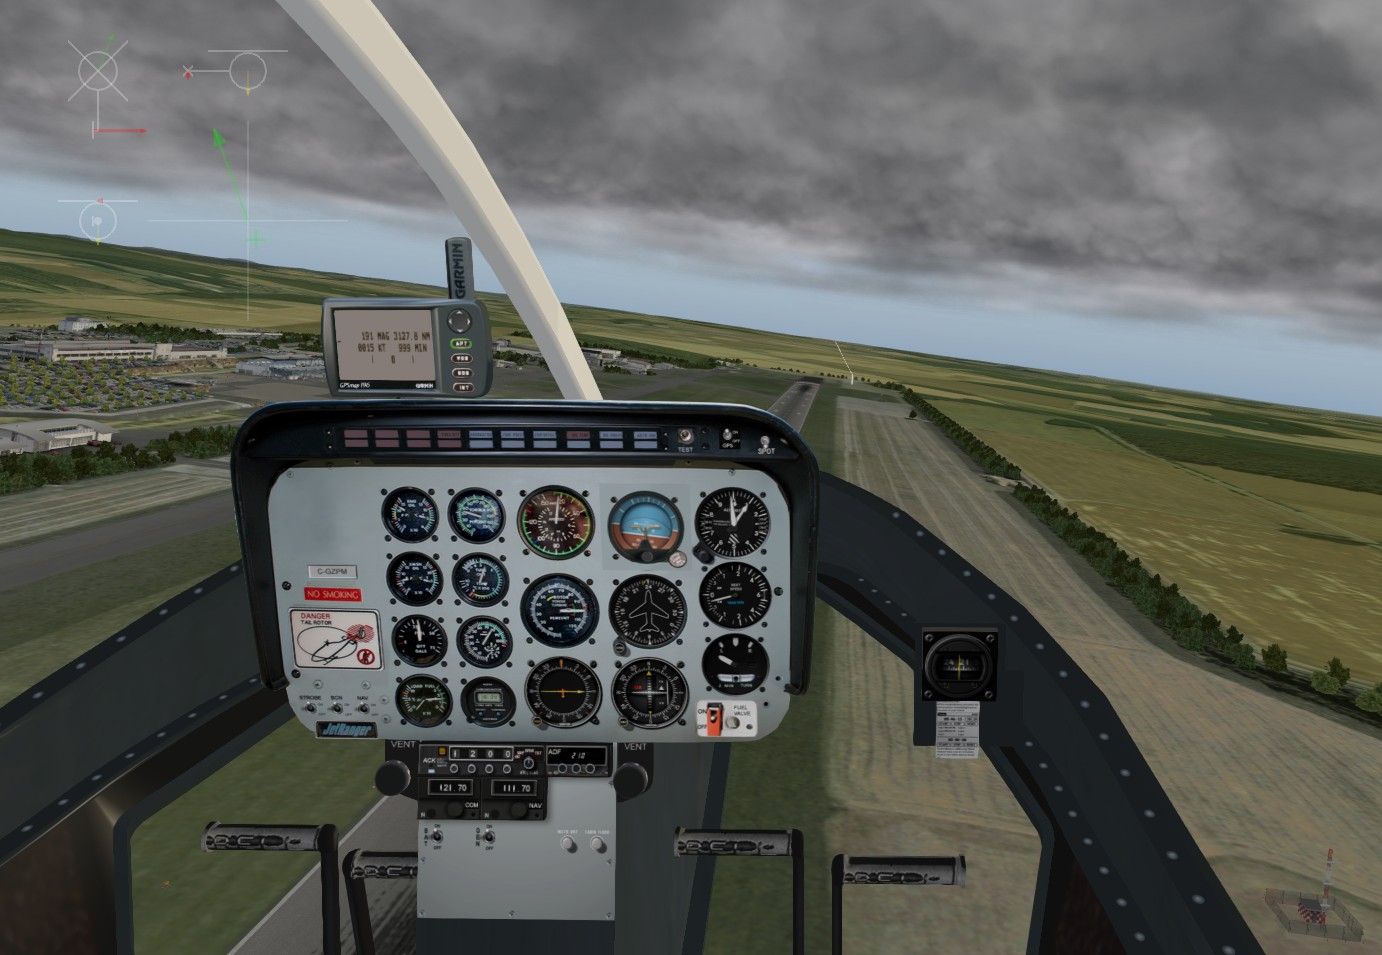
\includegraphics[width=14cm]{Jetranger_HeliTrim_EDLP.jpg}

To toggle if it should be displayed or not, you can assign a joystick command. The command is >>\verb|FlyWithLua/HeliTrim/show_toggle|<<.

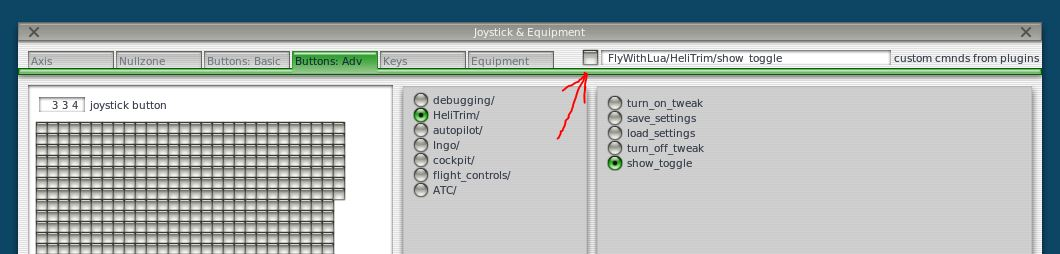
\includegraphics[width=14cm]{Assign_Heli_Display.jpg}

Just assign it to a joystick button or a key on your keyboard as shown in the picture above.

If you can't see the HeliTrim commands, click on the glassy looking button (marked above with the red arrow), then choose \verb|FlyWithLua|, \verb|HeliTrim| and \verb|show_toggle| from the list.

Now you can turn on or off the diagnostic display.

\subsection{The info provided by the display}

Let's take a deeper look onto the diagnostic display.

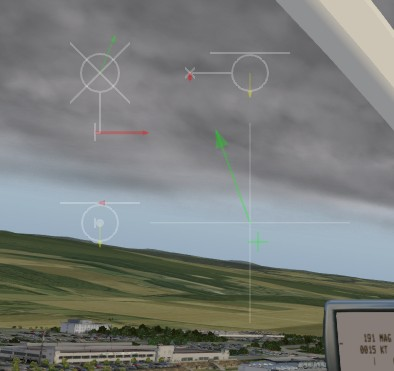
\includegraphics[width=10cm]{HeliTrim_zoom.jpg}

You find your helicopter drawn by some white lines. The helicopter is displayed from above, looking down to the helicopter, and also looking from the right side and from behind.

Colored arrows are showing the movement and the position of your sticks.

\textbf{The red arrows are showing the spinning speeds of your helicopter.}

As you can see in the example, the helicopter is spinning around his z-axis (yaw) to the left. This is shown by the long red arrow located at the tail rotor.

As we are flying a Bell 206 JetRanger, the tail rotor blades' angle is too low, allowing the main rotor to twist the helicopter.

Roll and pitch spinning is nearly zero.

\textbf{The yellow arrow is showing the VVI.}

Here the helicopter is going down. You can read the same info at the helicopter's panel.

\textbf{The little green arrow is showing the groundspeed and heading relative to the helicopter.}

In the example, we are drifting to the right side. Is the pilot drunken? He let's the tail rotor force a turn to the left. As the helicopter gets it's heading turned to the left, the drift to the right will disappear. There is a nice crosswind blowing from the south.

\textbf{The big cross with the green arrow and little green cross is showing the stick's position.}

The big green arrow is showing the position of the rudder pedals. The pilot kicks a little bit more into the left pedal.

The little green cross is showing the cycle stick position. As you can see in the example, the pilot is pulling the stick a little bit to his right leg.

\textbf{The white area is showing the range of the trim system.}

X-Plane's Bell 206 JetRanger doesn't have a trim system, so you do not see any white area. But load a C172, and you will guess what it is showing.

\textbf{The magenta arrow and cross is showing the trim system state.}

Again, without a trim system, you see nothing. But take a look onto the following picture. It is pretty mis-trimmed, but you can see how the display is working.

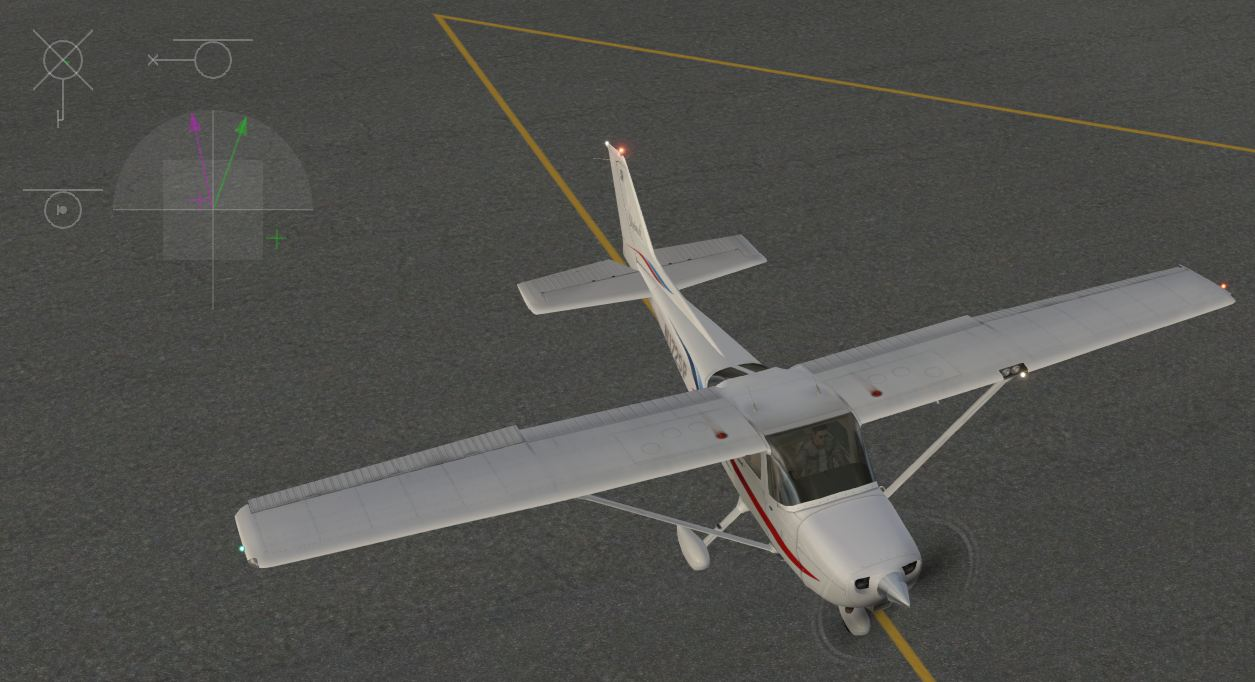
\includegraphics[width=14cm]{C172_trim_display.jpg}

Now, fly around with some of your planes and helicopters, and observe the diagnostic display.

\section{Trimming a helicopter}
\subsection{Trimming isn't Trimming}

A helicopter in X-Plane doesn't have a trim system. This is no surprise, as real helicopters do not have a trim system - why should X-Plane simulate it?

But a real helicopter has a cycle stick without a center position. You will have to use the same physical force on the real helicopter stick in every position around the center. But your joystick is using springs to keep the stick centered.

Using a >>Twister-Stick<< like the Thrustmaster T16.000M, instead of real helicopter sticks and pedals, is a pain to your hand, when flying a helicopter in X-Plane. You will have to permanently fight against the springs of the joystick, who are trying to force the stick back into it's neutral position (that isn't the real neutral position to fly the helicopter).

To avoid pain in your wrist, HeliTrim will help you.

\subsection{A new center}

Go into the advanced joystick button configuration and assign the command:\\ \verb|FlyWithLua/HeliTrim/turn_on_tweak|.

Then change the place of your helicopter in X-Plane to 10~nm to the next runway. This will put you into the air with engines running. As an alternative, you can start and lift off, if you like.

Fly strait forward and hold altitude. You will see, that you are not in the physical central position of your stick, but your helicopter is perfectly leveled out in the air (depending on your skills).

Now press and hold the button, you just assigned to \verb|FlyWithLua/HeliTrim/turn_on_tweak|. It is important that you hold the button down, or you will be surprised by the behavior of the helicopter.

While you hold the button down, the steering commands to X-Plane are frozen to the position, the joystick had at the moment, when you started pressing the button.

Bring the stick to his physical center and then release the button. Now get your hand off the stick and observe your helicopter. If you leveled him well, he should still fly strait forward and hold the altitude.

If you take a look at the diagnostic display, you see what happened. You will have a new center. If you now move your stick, all movements from the joystick's physical center are translated to X-Plane as movements from the just defined >>logical center<<.

And please remember, the diagnostic display is only for learning, the HeliTrim magic works independent from the display. This is the reason, why the diagnostic display is off by default. If the HeliTrim magic is working, a small text on top of the screen will indicate that it's really running.

\subsection{Adjusting the logical center}

Okay, let's change the speed you are flying. Changing speed will make it necessary to redefine the logical center. It's easy, just find the new logical center, press and hold the button again, move the stick to the physical center and release the button. You can do this as often as needed.

\subsection{Keeping a logical center in memory}

If you start your flight and hover to the runway (because the airport didn't have a helipad), you use a logical center. Lift off from the ground to hover is typically done like this. Pull the collective very smoothly and use the pedals to keep the heading (when raising the torch of the main rotor, the helicopter wants to twist around). But fighting against the twist with the tail rotor makes a pushing force to the side. To avoid drifting away, you need to slightly move the stick away from the center to the left or right, depending on the spinning direction of the main rotor.

If you found the right steering for a perfect hover, you can press the activation button to create a logical center made by HeliTrim.

HeliTrim offers two additional commands:\\
\verb|FlyWithLua/HeliTrim/save_settings|\\
and\\
\verb|FlyWithLua/HeliTrim/load_settings|

You guess what they are made for? Use the save command to store the logical center position into memory. If you fly a little traffic circuit and want to hover back to your parking position, you must find the perfect hovering setting again, as you changed the logical position during your flight.

Or you just use the load command -- and get it done much quicker.

\section{Advanced usage}

The following instructions are showing some programming in Lua. If you have absolutely no skill in programming a computer, stop reading this manual here and enjoy HeliTrim.

\subsection{Creating pre-defined settings}

Some helicopter have a similar trim system included as an in-plane plugin, but the big advantage of FlyWithLua is, that you can edit the code!

If you want pre-defined settings, there is a function provided in Lua:

\verb|set_heli_tweak_on(elv, ail, rud)|

To create the setting, we first need to find out the right values. It's easy, just save the settings into memory and look into the Log.txt file in X-Plane's main folder. You will find a line like this:

{\footnotesize\verb|FlyWithLua info: HeliTweak axis positions saved (elv = 0.036126, ail = -0.002439, rud = -0.146470)|}

Now take a text editor of your choice and start an empty (pure ASCII, not Word!) text file. Name it >>\verb|zzz_My_Heli_Settings.lua|<< and save it inside the \verb|Scripts| folder of FlyWithLua. It should start with >>zzz<< to be loaded and executed by Lua \emph{after} the \verb|HeliTrim.lua| script, as it uses functions that are declared inside \verb|HeliTrim.lua|, otherwise you get an undefined (unknown) function error.

Then fill the new script file like this\footnote{Lines beginning with >>~-~-~<< (two minus) are comments. Lua will ignore them and you can leave them away or edit them as you like.}:

\begin{lstlisting}[firstnumber=1]
-- My own heli trim stettings
-- --------------------------

-- Agusta Westland AW139 by X-Rotors
if PLANE_ICAO == "A139" then
  create_command("FlyWithLua/HeliTrim/hover_config", "set_heli_tweak_on(0.036, -0.002, -0.146)", "", "")
  create_command("FlyWithLua/HeliTrim/cruise_config", "set_heli_tweak_on(-0.029, 0.019, -0.106)", "", "")
end

set_button_assignment( 331, "FlyWithLua/HeliTrim/hover_config" )
set_button_assignment( 332, "FlyWithLua/HeliTrim/cruise_config" )
\end{lstlisting}

Now your buttons no. 331 and 332 load a pre-defined setting and turn on the HeliTrim tweak.

\subsection{Helping the community}

If you made a perfect set of settings for one or more helicopters in X-Plane, please share it with the community. You can upload it to \href{http://forums.x-plane.org/index.php?app=downloads&showcat=9}{x-plane.org} or send it to me via email and I will integrate it into FlyWithLua.

\subsection{Change stick sensitivity}

Most helicopter pilots don't like a non-linear behavior of the stick. By default HeliTrim uses a 1:1 linear translation from the sticks angle to the addition on the logical center. You might say, a 1:1 translation is much to fast to fly a helicopter.

There is a variable in Lua, you can change. Complete your little config script with this line:

\begin{lstlisting}[firstnumber=12]
HeliTrim_sensitivity = 0.5
\end{lstlisting}

Now you can move the stick to it's end, but X-Plane will see only a half movement instead of a full movement. Use the diagnostic display to see how it is working. And find a good value for your own device. It's a compromise between fine and heavy movement, depending on the type of the helicopter and your flying style. A small value is good for smooth flights, a value near 1.0 allows riding the beast like a wild horse.

\end{document}
\endinput
